\documentclass[12pt]{article}
\usepackage[utf8]{inputenc}
\usepackage{amsmath}
\usepackage[spanish]{babel}
\usepackage{csquotes}
\usepackage{biblatex}
\addbibresource{bibliografia.bib}
\usepackage{graphicx}
\graphicspath{ {images/} }

\title{
    {Patrones de sincronización y disparo en mapas neuronales acoplados de Rulkov}\\
    {\large Universidad de Buenos Aires}\\
    {\large Facultad de Ingeniería}\\
    \vspace{0.8cm}
    {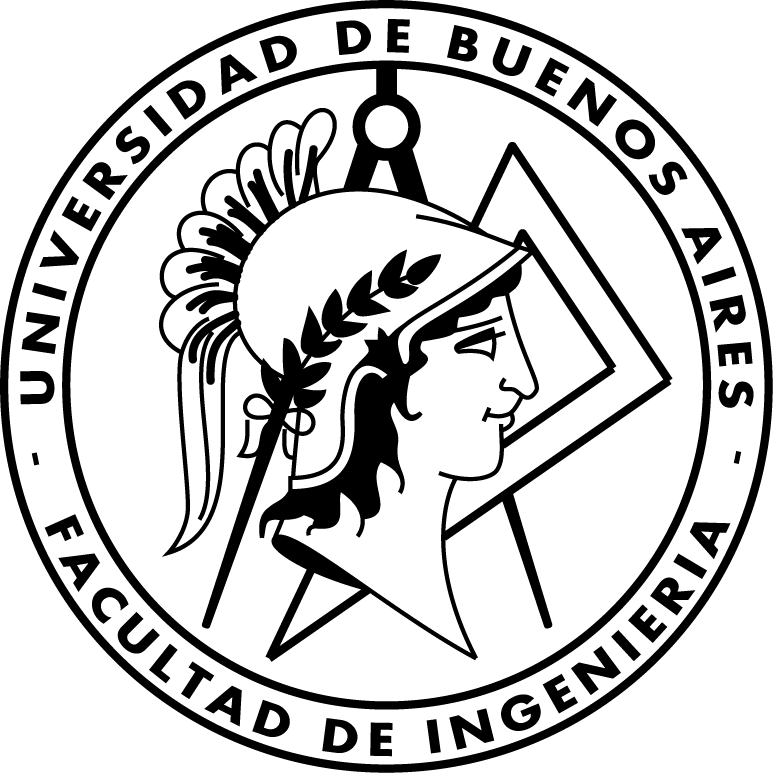
\includegraphics{logo_fiuba.png}}
}
\author{Nicolás Gatti}
\date{2020}

\begin{document}

\begin{titlepage}
\maketitle
\end{titlepage}

\section{Introducción}

\subsection{Sincronización Neuronal}

Dentro del área de las neurociencias, el estudio de la sincronización neuronal es un area muy interesante, ya que mediante la misma se busca explicar el mecanismo por el cual el cerebro transmite y codifica información. 

En un principio se creía que el cerebro se organizaba en una estructura jerárquica y que algunas neuronas especializadas se ocupaban de tareas especificas, mientras que las demás se ocupaban de transmitir la información, sin embargo, este modelo implicaba que la cantidad de neuronas necesarias era mayor del observado. 

En la actualidad, se cree que las neuronas en realidad funcionan en forma descentralizada y que las mismas tienen la capacidad de sincronizarse espontáneamente para realizar tareas especificas. De esta forma el cerebro tiene la capacidad de realizar tareas en paralelo haciendo trabajar en conjunto las partes necesarias cada vez.

Más aún, se han encontrado evidencias de que algunos desordenes neurológicos como el Parkinson, Alzheimer o epilepsia se deben a patologías que alteran la normal sincronización de las neuronas.

\subsection{Objetivo}
El presente trabajo tiene como objetivo analizar la estabilidad de la sincronización neuronal en redes neuronales de Rulkov. Mediante análisis de estabilidad del punto fijo se establecerán las condiciones de estabilidad de dicho sistema.

\section{Modelo matematico estudiado}
Para estudiar los estados dinamicos colectivos de los sistemas neuronales acoplados se utiliza el modelo de Mapa de Rulkov no lineal de dos dimensiones, ya que se demostrará que este modelo es capaz de reproducir diferentes tipos de patrones de disparo observados en las neuronas que incluyen spiking, bursting y silent state.

El modelo parte del modelo de oscilador propuesto por Rulkov en \cite{rulkov}, pero para poder evidenciar el comportamiento de sincronizacion agrega los efectos de la sinapsis quimica y el acoplamiento interno entre dos neuronas.

\subsection{Variables de Estado}
El modelo matematico de 2 mapas de Rulkov acoplados en presencia de sinapsis quimica y acoplamiento interno es el siguiente: 

\begin{align} \label{Rulkov_map}
\begin{split}
x_{1}(n+1) = &f(x_{1}(n),y_{1}(n),\alpha_{1}) \\
             &+ g_{c}(v_{s}-x_{1}(n))\Gamma(x_{2}(n)) \\
             &+\epsilon[f(x_{2}(n),y_{2}(n),\alpha_{2})-f(x_{1}(n),y_{1}(n),\alpha_{1})]  
\end{split}
\\
y_{1}(n+1) = &y_{1}(n)-\eta(x_{1}(n)-\sigma)
\\
\begin{split}
x_{2}(n+1) = &f(x_{2}(n),y_{2}(n),\alpha_{2}) \\
             &+ g_{c}(v_{s}-x_{2}(n))\Gamma(x_{1}(n)) \\
             &+\epsilon[f(x_{1}(n),y_{1}(n),\alpha_{1})-f(x_{2}(n),y_{2}(n),\alpha_{2})]  
\end{split}
\\
y_{2}(n+1) = &y_{2}(n)-\eta(x_{2}(n)-\sigma)
\end{align}

Donde:: 
\begin{equation*}
f(x_{i}(n),y_{i}(n),\alpha_{i}) = \frac{\alpha_{i}}{1+x_{i}^{2}}+y_{i}
\end{equation*}

Siendo el tercer termino de las ecuaciones 1 y 3 el efecto del acoplamiento interno. 

El parámetro $\sigma$ representa una corriente continua externa suministrada a la neurona, $\alpha_{i}$ es un parámetro de control que regula los diferentes tipos de patrones de disparo. 

La funcion de acoplamiento sinaptico quimico es representada en la ecuacion por: 
\begin{equation*}
\gamma(x) = \frac{1}{1+e^{-k(x-\Theta_{s})}}
\end{equation*}

Finalmente, la variable de estado $x_{i}(n)$ representa el potencial trans-membrana de la neurona i-ésima en el paso discreto n, mientras que $y_{i}(n)$ identifica la corriente de recuperacion ionica y posee una variacion dinámica lenta debido al valor de $\eta (0 < \eta << 1)$.

\subsection{Parámetros del sistema}
Los parametros $\alpha$ y $\sigma$ determinan si el sistema se encuentra en descanso, spiking o bursting. Para la simulacion se define $\alpha_{1}=\alpha_{2}=\alpha=4.1$ y $\sigma=-1.6$. 

Mientras tanto, $\epsilon$ y $g_{c}$ representan la fuerza de acoplamiento interno y quimico sináptico, respectivamente. Estos comportamientos identifican como se transimite la informacion entre las dos neuronas que interactúan en el modelo.

El potencial $v_{s}$ es el potencial sinaptico inverso, cuando $v_{s}$ es mayor a $x_{i}(n)$ se dice que la sinapsis es excitatoria, mientras que en el caso contrario es inhibitoria. En la simulación $v_{s}=-1.4$

En referencia a la funcion $\Gamma$, la misma se comporta como una funcion sigmoide, el parametro $k$ regula el slope de la funcion, mientras que $\Theta_{s}$ regula el disparo. Estos parametros son fijados en los siguientes valores: $k=50$ y $\Theta_{s}=-1.4$

Por otro lado el parametro $\eta$ se fija en 0.001.

\section{Analisis de punto fijo y estabilidad lineal}
Dado que el sistema es no lineal, se procede a describir el comportamiento local en las proximidades del punto fijo.

El sistema descripto posee un unico punto fijo definido por: 

\begin{equation}
    P = (\sigma, \sigma - \frac{\alpha}{1+\sigma^{2}} + \frac{g_{c}(\sigma-v_{s})}{1+e^{-k(\sigma-\Theta_{s})}}, \sigma, \sigma - \frac{\alpha}{1+\sigma^{2}} + \frac{g_{c}(\sigma-v_{s})}{1+e^{-k(\sigma-\Theta_{s})}})
\end{equation}

Se puede observar que no hay efecto de la fuerza de la funcion de acoplamiento interno $\epsilon$ en la posicion del punto fijo

\medskip

\printbibliography

\end{document}
